\documentclass[12pt,a4paper]{article}

% Margins.
\setlength{\oddsidemargin}{0in}
\setlength{\evensidemargin}{0in}
\setlength{\headheight}{12pt}
\setlength{\headsep}{42pt}
\setlength{\topmargin}{-54pt}
\setlength{\textwidth}{6.5in}
\setlength{\textheight}{10in}

\usepackage{amsmath}
\usepackage{float}
\usepackage{graphicx}
\usepackage[hyphens]{url}
\usepackage{hyperref}	% Clickable links to figures, references and urls.
\usepackage{datetime}
\usepackage{longtable}

% Links direct to top of figures.
\usepackage[all]{hypcap}

% Drawing.
\usepackage{pgf}
\usepackage{tikz}

% Listings for formatting code.
\usepackage{listings}
\usepackage{textcomp}
% General options.
\lstset{breaklines=true, basicstyle=\small\ttfamily, tabsize=4, numbers=left, stepnumber=1, frame=single, showstringspaces=false, upquote=true}
% C++ specific high-lighting. Comments are 50/50 shades of green/black and strings coloured with 60/40 red/black mixture.
\lstset{language=[ISO]C++, commentstyle=\color{green!50!black}, keywordstyle=\color{blue}, stringstyle=\color{red!60!black}}

%opening
\title{\vspace{-2cm}Physics for Engineers\\Class 09\\Line, Surface and Volume Integrals}
\author{Attique Dawood}
\date{September 06, 2013\\[0.2cm] Last Modified: \today, \currenttime}
\begin{document}
\maketitle
\section{Announcements}
\begin{itemize}
\item None.
\end{itemize}
\section{Revision}
\begin{itemize}
\item Differential length, surface and volume elements.
\end{itemize}
\section{Surface and Volume Integrals}
In electromagnetics we need to solve surface and volume integrals. Some common integrals are given below.
\begin{itemize}
\item $\int_{S} d\mathrm{A}$~: Gives the total area of the surface `S'. This is generalised expression actually solved as a double integral.
\item $\int_{v} dv$~: Calculate the total volume defined by limits of `v'. This is also a generalised expression actually solved as a triple integral.
\item $\int_{S}\textbf{A}\cdot d\textbf{A}$~: Gives the total flux of the vector field \textbf{A} through the surface `S'.
\item $\int_{v}\rho_v dv$~: If $\rho_v$ is volumetric charge density in $C/m^3$ then this integrals gives the total charge in volume `v'.
\end{itemize}
\section{Introduction to the Line Integral}
Line integral is the generalisation of single variable integral. You may have only seen integrals of the kind $\int_{x=a}^{x=b} f(x)dx$ till now. The path of this integration is along the $x$--axis from $x=a$ to $x=b$. In electromagnetics we come across integrals where the path of integration may be any arbitrary (curved or zig zag) path in 3D space. Two important line integrals are
\begin{itemize}
\item $\int_{a}^{b}\hat n\cdot d\textbf{\textit{l}}$~: Gives the length of the path from a to b if $\hat n$ is parallel to the path.
\item $\int_{a}^{b}\textbf{A}\cdot d\textbf{\textit{l}}$~: If \textbf{A} is force, then this integral gives the total work done from a to b. If \textbf{A} is electric field then this integral gives potential difference (or voltage) between a and b.
\end{itemize}
Notice, these integrals give a scalar. There are other forms of line integrals but we will restrict ourselves to these two for now.
\section{Using Calculator to Solve Integrals}
A calculator can be used to solve definite integrals. To find $\int_{0}^{3}x^2dx$, the key sequence is: $\boxed{\int dx}$ $\boxed{ALPHA}$ $\boxed{X}$ \fbox{\textasciicircum} $\boxed{2}$ $\boxed{,}$ $\boxed{0}$ $\boxed{,}$ $\boxed{3}$ $\boxed{)}$ $\boxed{=}$. The answer should come out to be 9. The sequence of instructions is: integration notation followed by expression to integrate and then limits of integration. On newer models limits may be entered in boxes.

It is important to note that the calculator only treats `X' as the variable of integration. So, if you need to evaluate $\int_{0}^{3}t^2dt$, the expression would be the same as above replacing t with `X' during input.
\section{Exercises}
\noindent\textbf{Question 1:} Use an appropriate $dS$ to find the surface area of given structures.
\begin{itemize}
\item[(1)] The area of curved surface of a cylinder of radius, $\rho=3$ and height 2.
\item[(2)] The surface area of a sphere of radius, $r=3$.
\item[(3)] The area of curved surface of a slice of cake described by $\rho=3$, height 2 and $0<\phi<30^0$.
\item[(4)] The area of an icecream cone described by $\theta=30^0$ and $0<r<3$.
\end{itemize}
\noindent\textbf{Question 2:} Use a suitable $dv$ to find the volumes of structures given in question 1.\\[0.2cm]
\noindent\textbf{Question 3:} Using $\int_{a}^{b}\hat n\cdot d\textbf{\textit{l}}$
\begin{itemize}
\item[(1)] Find the length of line segment from (0, 0) to (1, 2). Solve this in Cartesian as well as Cylindrical coordinates.
\item[(2)] Find the length of body/space diagonal of a unit cube.
\item[(3)] Find the arc length of a quarter circle of radius $\rho=3$ m in first quadrant.
\item[(4)] Find the length of the curve $y=x^2$ from (0, 0) to (1, 1). For this problem a calculator would be handy in solving the integrals.
\end{itemize}
\noindent\textbf{Note:} For part (4) you need to find a unit vector along the curve $y=x^2$. A vector parallel (or tangent) to $y=x^2$ can be obtained from the slope. Numerator and denominator of slope ($\dfrac{dy}{dx}$) are the $y$-- and $x$--components, respectively, of the vector. Here, $\dfrac{dy}{dx}=\dfrac{2x}{1}$ so the parallel/tangent vector is $\textbf{n}=\hat x+2x\hat y$. The unit vector is then $\hat n=\dfrac{\hat x+2x\hat y}{\sqrt{1+4x^2}}$.\\[0.2cm]
\newpage
\noindent\textbf{Question 4 (Example 2--4C \cite[Example 2--4, page 23]{Cheng}):} Given a force field $\textbf{F}=xy\hat x+(3x-y^2)\hat y$ in a region, evaluate the integral $\int_{P1}^{P2}\textbf{F}\cdot d\textbf{\textit{l}}$ to find the total work done in moving from P1 to P2 along path 1 and path 2.\\[0.2cm]
\noindent\textbf{Question 5:} Electric field in a region is $\textbf{E}=x\hat x+y\hat y$. Refer to figure \ref{Cheng-integral}, evaluate the integral $\int_{P1}^{P2}\textbf{E}\cdot d\textbf{\textit{l}}$ to find the potential difference between P1 and P2. Is the potential difference same for path 1 and path 2?
\begin{figure}[H]
\centering
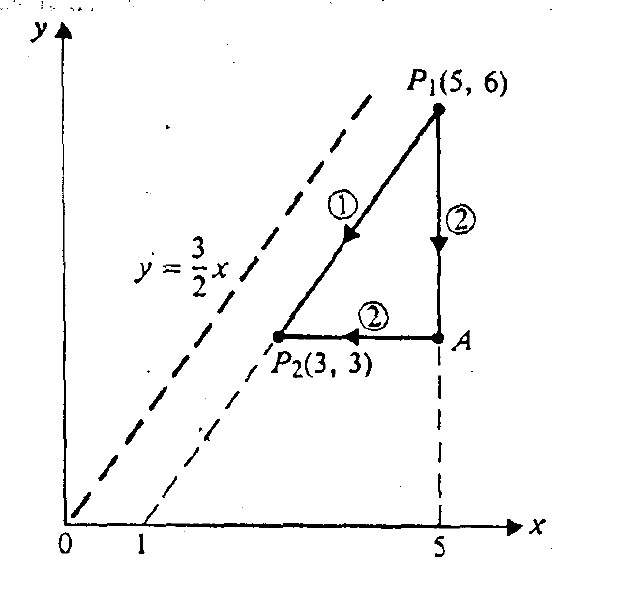
\includegraphics[scale=0.6]{Figure2-10Cheng.png}
\caption{Paths of integration for Question 2 \cite[Figure 2--10, page 23]{Cheng}}
\label{Cheng-integral}
\end{figure}
%\nocite{*}
\bibliographystyle{plain}
\bibliography{PhysicsRef}
\end{document}
